\section{Reactors} \label{sec:reactors}
Nine designs of micro-reactors are under investigation: Westinghouse (eVinci), Holosgen (Holos), \gls{LANL} (MegaPower), MicroNuclear, NuScale (NuScale), Oklo (Oklo), Starcore (Starcore), Urenco (U-battery) and X-energy (Xe-100) (in alphabetical order). Kairos does not have any reactor designs which produce power less than 200 MWe. A brief comparison of the selected reactors is listed in Table \ref{microreactors-1} and \ref{microreactors-2}. In addition, recent progresses in the design reviews of different reactors around the world are provided in Table \ref{reviews}. 

The information on reactor designs was mainly gathered from the following sources.

1. International and domestic government organization databases: design information was collected from the \gls{IAEA} , the \gls{NEA}, the \gls{DOE}, and the NRC online databases.

2. Vendor database: the latest design brochures, catalogs and reports were directly obtained from the vendors.

Notes:

1. \gls{GA} is developing a mobile nuclear power supply that is truck/air shippable and would fit in a standard military shipping container. This modular, autonomous system has a load-following generating capacity of up to 10 MWe and a refueling period greater than 10 years. (source: press releases)

2. The NuGen Engine developed by NuGen is a direct-cycle gas-cooled microreactor. The concept design, by Professor Tsvetkov at the Department of Nuclear Engineering at Texas A$\&$M University, produces 1-50 MWe scalable output. It is in the stage of patent aproaval. (source: https://www.nucdev.com/about-us.html)

3. In the case of \gls{MSR} design at micro-level, only Terrapower has started to adopt its \gls{MCFR} design to 1-10 MWe with more than 10 years refueling.(source: press releases of the president) 

\pagebreak
\newgeometry{margin=1cm}
\begin{landscape}
\begin{table} [ht]
\begin{center}

\caption{A brief comparison of micro-reactor designs -1}
\label{microreactors-1}
\begin{tabular}{|l|l|l|l|l|l|l|l|l|l|}
\hline 
Design 		&eVinci 		& Holos		&MegaPower 	& NuScale		& Oklo 		& Starcore		 \\ 
\hline 
Institution 	&Westinghouse& Holosgen	&LANL	& NuScale		& Oklo Inc. 	& Starcore		\\ 
Source 	&\cite{levinsky_westinghouse_2018};\cite{yan_technology_2020};\cite{arafat_evinci_2019}  &\cite{filippone_holos_2017}  	& \cite{mcclure_design_2015};\cite{sterbentz_special_2017}	& \cite{nuscale_chapter_2018} 		& \cite{oklo_inc._pilot_2018} 	&vendor's website		\\ 
Type			&Heat Pipe	& HTGR (Pebble)	  	& Heat Pipe 		& PWR/Heat Pipe&Heat Pipe   			&	HTGR (Pebble)			\\ 
Spectrum		&Epithermal	& Thermal 		 	&Fast  	&Thermal/Thermal 		&Fast   			& Thermal  			\\ 
Power (MWe)	&0.2-5		& 10/13  			&2			& 10-50 /1-10			& 2  			&2x10  			\\ 
Refueling (years)&5 to 10		&12 or 20   			&	5		& 2/- 			& up to 20  			&5  			\\ 
Enrichment (\%)&19.75		&8 for 12 or 15 for 20   			&19.75			& $<$4.95/- 		&  5 to 20 			&$<$20	  			\\ 
Core  Diameter (m)	&1.5		& 1.8  			&1.5			& 1.5/- 		&   			&1.5   			\\ 
Fuel			&UN/U-Mo	& UCO TRISO  			&	UO2		&UO2/-		&  U-Zr 			& UCO TRISO  			\\ 
Clad			&-		&  Silicon carbide 			&	-		& M5/- 		&   -			&Silicon carbide   			\\ 
Heat Pipe fluid	&Na/K	& -  			&K			& - 		& Na/K 			&  - 	\\ 
\hline
\end{tabular}

\caption{A brief comparison of micro-reactor designs -2}
\label{microreactors-2}
\begin{tabular}{|l|l|l|l|l|l|l|l|l|l|}
\hline 
Design 		& Hydromine & U-battery 	& MMR 	& Xe-100 \\ 
\hline 
Institution  & Hydromine & Urenco 	& USNC	& X-energy \\ 
Source 			& - &\cite{ding_design_2011}  	&\cite{venneri_neutronic_2015} 	&\cite{iaea_advances_2018}; \cite{harlan_x-energy_2018} \\ 
Type			&  LFR & HTGR (Pebble)	& HTGR (Pebble) & HTGR (Pebble)\\ 
Spectrum	& Fast	&	Thermal		&Thermal &Thermal\\ 
Power (MWe)	  	& 5		&4-8		&5	&75\\ 
Refueling (years) & 15 &5-10 	&20		&Online refueling\\ 
Enrichment (\%)  &19.75 &20-17	&12		&15.5\\ 
Core  Diameter (m)&- &3.5-1.8		& 3 	& 4.88 (RPV)\\ 
Fuel			& UO2&UCO TRISO	&UCO TRISO	&UCO TRISO\\ 
Clad			& -&Silicon carbide		&Silicon carbide 	&Silicon carbide\\ 
Heat Pipe fluid	&-&	-			&	-		&-\\ 
\hline
\end{tabular}

*\gls{HTGR}, \gls{PWR}, \gls{RPV}, \gls{TRISO}
\end{center}
\end{table}
\end{landscape}
\restoregeometry
\pagebreak

\newgeometry{margin=1cm}
\begin{landscape}
\begin{table} [ht]
\begin{center}

\caption{Worldwide design reviews}
\label{reviews}
\begin{tabular}{|l|l|l|l|l|l|}
\hline 
	 &Country of Origin 	& Company		&Reactor type			&Output(MWe) 	& Status \\ 
\hline 
1 	&Canada/US		& Terrestrial Energy	&Molten Salt Integral	&200		& PHASE 1 COMPLETED \\ 
 	&		& 	&	&		& PHASE 2 PENDING  \\
2 	&US/Korea/China	& UltraSafe Nuclear	&High-temperature gas prismatic block	&5		& PHASE 1 IN PROGRESS completion date 2018   \\ 
 	&		& /Global First Power	&	&		& PHASE 2 Service Agreement under development  \\
3 	&Sweden/Canada	&LeadCold	&Molten lead pool fast spectrum	&3-10		& PHASE 1 ON HOLD AT VENDOR REQUEST  \\ 
4 	&US		&Advanced Reactor Concepts	&Sodium pool fast spectrum	&100		& PHASE 1 IN PROGRESS  \\ 
5 	&UK		&U-Battery	&High temperature gas prismatic block	&4		& PHASE 1 Service Agreement under development  \\ 
6 	&UK		&Moltex Energy	&Molten salt fast spectrum	&300		& PHASE 1 IN PROGRESS  \\ 
7 	&Canada/US		&StarCore Nuclear	&High-temperature gas prismatic block	&10		& PHASE 1 and 2 Service Agreement under development   \\ 
8 	&US		&SMR, LLC. &Pressurized Water	&160		&PHASE 1 Service Agreement under development   \\ 
 	&		& (A Holtec International Company)		&	&		&  \\
9 	&US		&NuScale Power	&Integral Pressurized Water	&50		&PHASE 2* Service Agreement under development   \\ 
10 	&US		&Westinghouse Electric Co.	&eVinci Micro Reactor	&$<$25		&PHASE 2* Service Agreement under development  \\ 
11 	&Japan		&4S	&Na cooled fast reactor	&10		&Licensing pre-application  \\ 
12 	&Russia		&ABV	&PWR	&2x7.9		&Part of design licensed  \\ 
13 	&Argentina	&CAREM-25	&PWR	&27		&Licensing in progress  \\ 
14 	&Russia		&KLT-40S	&PWR	&2x35	&Licensed and under construction  \\ 
\hline

\end{tabular}

\end{center}
\end{table}
\end{landscape}

\restoregeometry
\pagebreak

\subsection{GA}
EM2 (Energy Multiplier Module) is 500 MWt / 265 MWe gas cooled reactor (GCR), fast spectrum, the fuel form and enrichment are not disclosed. The primary coolant is forced circulation helium, core outlet temperature 850 $^{\circ}$C. The core lifetime is 30 years. The power conversion cycle is not specified.

\subsection{Holosgen}
Holos design uses four subcritical fuel cartridges as given in Fig. \ref{Holosquad}. TRISO fuels fill the fuel channels, as illustrated in Fig. \ref{Holosdesign}. Complete design details including radiation protection and shielding, and safety are available in \cite{filippone_holos_2017}.

\begin{table} [htbp]
\begin{center}

\caption{Holos core geometry and composition}
\label{Holostable}
\begin{tabular}{l     l}
\hline 
Design 		&Value \\ 
\hline 
Reactor thermal power (MWt)&22                                             \\
U-235 enrichment (wt\% )&8-15             \\
Whole core volume (m$^3$)&6.9                                        \\
\hline 
Fuel Channels&19x4                      \\
Fuel Channel Diameter (cm)&1.4            \\
Coolant Channels&54x4                   \\
Coolant Channel Diameter (cm)&0.7               \\
Brick Graphite Density (g/cm$^3$)&2.23              \\
Brick Edge Length (cm)&6               \\
Brick Height (cm)&10             \\
\hline 
UO2 Density  (g/cm$^3$) & 10.8                       \\
Kernel Diameter  (cm) & 0.05                       \\
Buffer Layer Thickness  (cm) & 0.01            \\
SiC, IPyC, OPyC Thickness  (cm) & 0.012   \\
TRISO Sphere Diameter  (cm) & 0.094         \\
Total core bricks & 1,925                           \\
Packing Fraction (\%) & 70                       \\
\hline 
TRISO spheres in one fuel channel  &24,778   \\
TRISO spheres in one brick            &470,777 \\
TRISO spheres in core  &3.62x10$^{9}$            \\
\hline 
Temperature Coefficient of Reactivity -$\rho_{T}$- (pcm)&-8       \\
Delayed Neutron Fraction -$\beta_{eff}$- (pcm)&733      \\
Generation Time -$\Lambda$- ($\mu$s)&233                        \\
\hline 

\end{tabular}
\end{center}
\end{table}

\begin{figure}[hbtp]
\centering
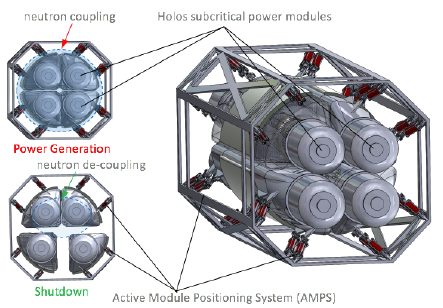
\includegraphics[scale=1]{Figs/holosquad.jpeg}
\caption{Holos Quad generator}
\label{Holosquad}
\end{figure}

\begin{figure}[hbtp]
\centering
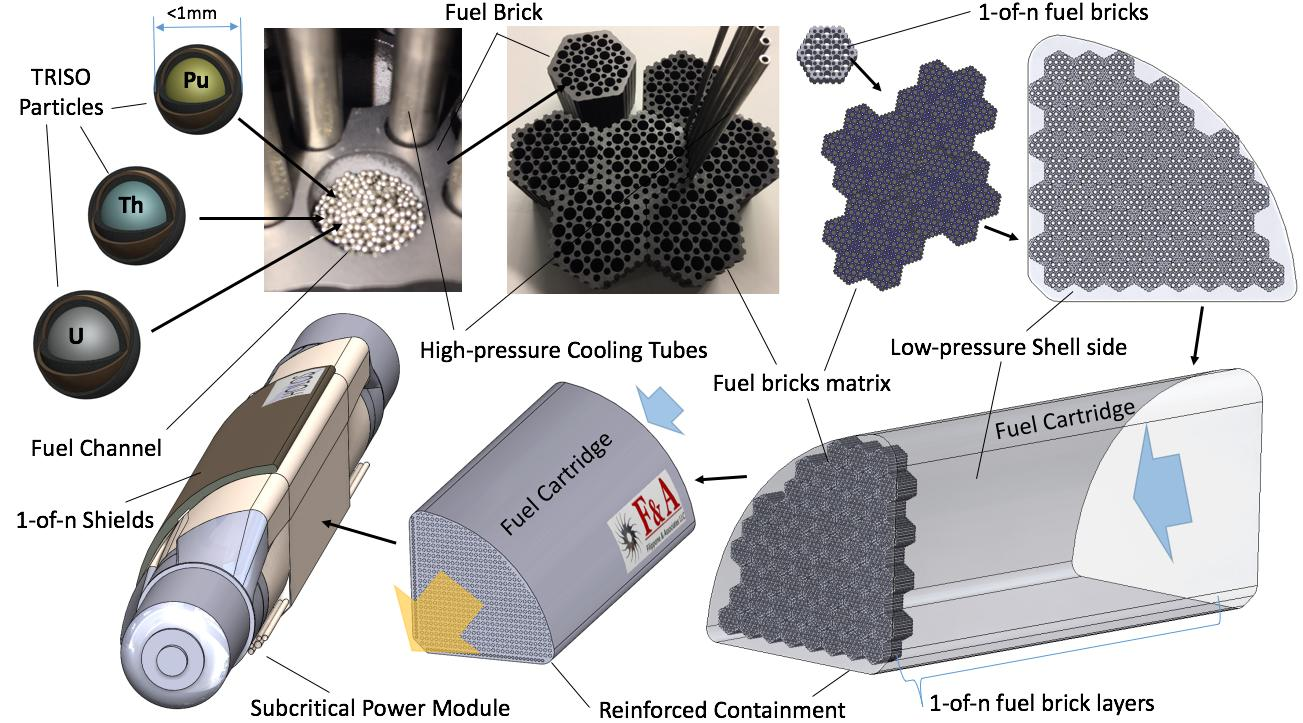
\includegraphics[scale=0.3]{Figs/holosfueldesign.jpeg}
\caption{Holos subcritical assembly design}
\label{Holosdesign}
\end{figure}

\pagebreak

\subsection{Hydromine}
LFR-TL (Transportable Long-life core) is a 15 MWt / 5 MWe lead cooled fast reactor (LFR), with UO2fuel,19.75\% enriched. The coolant is forced circulation lead, inlet/outlet temperature 360/420 $^\circ{}$C. The core lifetime is 15 years. The power conversion is a conventional steam cycle. LFR-AS (Amphora Shape) is a 480 MWt / 200 MWecommercial version of the reactor.

\subsection{Kairos  Power}
KP-FHR is  a  310  MWt  /  140  MWe  fluoride  salt  cooled  high-temperature  reactor  (FHR),  graphite moderated,  pebble  bed  UO2TRISO  fuel  (19.9\%  enriched). The  primary coolant  is  forced  circulation  fluoride  salt (Li2BeF4), system pressure 0.3 MPa, core inlet/outlet temperatures 600/700 $^\circ{}$C. On-line fueling allows for continuous operation, fuel pebbles pass through the core $\sim$ 8 times to achieve burn up to 180 GWd/tHM. The power conversion is a conventional steam cycle.

\subsection{LANL}
MegaPower is a LANL reactor design concept. Table \ref{Megatable} provides important features of MegaPower reactor parameters. More specific design details can be found in the reports \cite{sterbentz_special_2017} and \cite{mcclure_design_2015}. Results of the neutronics and thermal-hydraulics analyses have been published by \gls{INL} and LANL in various reports. Apart from a 5 MWt design, there is an advanced 15 MWt design which uses UN fuel and Na as HP fluid. However, publications are mostly on the first design shown in Figs. \ref{Megadesign} and \ref{Megaoverview}. 

\begin{figure}[hbtp]
\centering
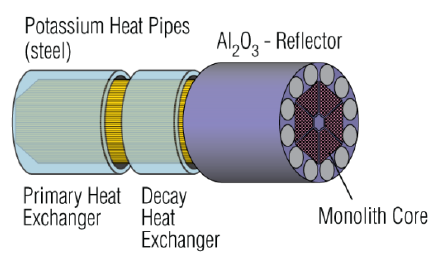
\includegraphics[scale=0.8]{Figs/megacore.jpeg}
\caption{Megapower concept design}
\label{Megadesign}
\end{figure}

\begin{figure}[hbtp]
\centering
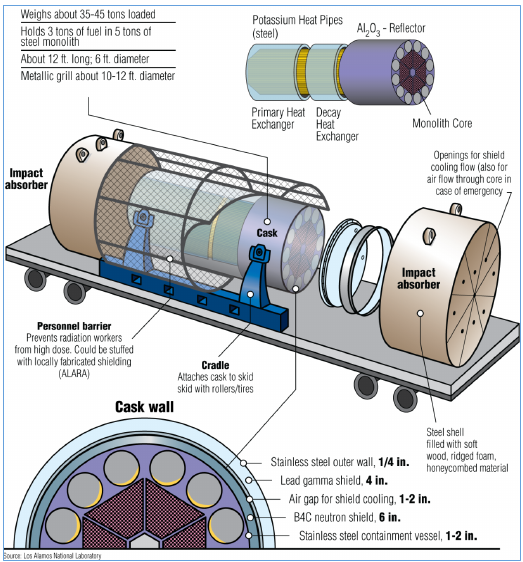
\includegraphics[scale=0.7]{Figs/megacask.jpeg}
\caption{Megapower reactor overview}
\label{Megaoverview}
\end{figure}

\pagebreak
\begin{table} [hbtp]
\begin{center}

\caption{MegaPower Reactor Core Description}
\label{Megatable}
\begin{tabular}{l     l}
\hline 
Design 		&Value \\ 
\hline 
Reactor thermal power&5 MW                                             \\
Reactor electrical power output&2 MW(e)                                       \\
Reactor core orientation&Horizontal                                       \\
Cycle length&5 years                                           \\
Coolant system&Heat pipes                                      \\
Reactor structure&Type 316 Stainless steel monolith    \\
\hline 
Fuel Form&UO2                      \\
Theoretical density&10.96 g/cm$^3$           \\
Percent of theoretical density&96.0\%                   \\
U-235 enrichment&19.75 wt\%             \\
Fuel channel hole outer diameter&1.425 cm               \\
Fuel pellet geometry&Cylindrical              \\
Fuel pellet outer diameter&1.412 cm               \\
Gas gap thickness&0.0065 cm             \\
Fuel rod length&150.0 cm               \\
Fuel-to-fuel pitch&1.60 cm                 \\
Fuel-to-HP pitch&1.60 cm                 \\
Gas&Helium                   \\
Gas pressure&20 atmospheres   \\
Number of fuel rods in-core&2,112                     \\
\hline 
Number of HPs in-core&1,224         \\
HP hole diameter (in-core)&1.575 cm    \\
HP-to-HP pitch&2.7713 cm  \\
HP working fluid&Potassium  \\
HP total length&4.0 m         \\
HP isothermal temperature&675$^\circ{}$C        \\
\hline 
Monolith material&Stainless steel (SS316)       \\
Monolith steel density&8.03 g/cm$^3$                         \\
Monolith edge thickness (HP-to-edge)&2 mm                                 \\
Web thickness between HP-to-fuel holes&0.100 cm                            \\
Web thickness between fuel-to-fuel holes&0.175 cm                            \\
Web thickness between HP-to-edge of block&0.150 cm                            \\
\hline 
Side reflector material&Alumina (Al2O3)       \\
Alumina density&3.9 g/cm$^3$                        \\
Side reflector outer radius&77.85 cm                                 \\
Side reflector radial thickness&21-29 cm                            \\
Top/bottom reflector material&SS316 + BeO                            \\
\hline 
Number of control drums&12       \\
Number of emergency control rods&2       \\
Control material&B4C                        \\
\hline 

\end{tabular}
\end{center}
\end{table}

\pagebreak
\subsection{MicroNuclear}
MsNB  (Micro-Scale  Nuclear  Battery)  is  a  10  MWe  heat  pipe  reactor  (HPR),  cooled  by sodium/potassium heat pipes, molten salt fuel (enrichment undisclosed). The core is molten salt (FLiBe) with dissolved fuel,  with  no  recirculation  outside  of  the  vessel.  The  reactor  can  operate  10  years  without  refueling.  The  power conversion is a Brayton cycle.

\subsection{Moltex Energy}
SSR (Stable Salt Reactor) is 375 MWt / 150 MWe molten salt reactor (MSR), fuel salt 60/40\% NaCl / AcCl3 (enrichment  not  reported). There  is  a  fast  and  thermal  (graphite  moderated)  version. The primary  coolant  is forced circulation 42/10/48\% ZrF4/NaF/KF, melting point 385 $^{\circ}$C. Core inlet/outlet temperature is 525/650 $^{\circ}$C. The molten salt fuel is stationary inside of a fuel pin, arranged as a lattice similar to LWR geometry. Fuel pins are inside of vessel with molten salt coolant. Fuel pins are open and allowed to vent fission gases, such configuration allows for high burnup  due  to  venting  of  fission  gases  and  axially  uniform  burn  due  to fuel salt  mixing. On-line  fueling  allows  for continuous operation. The power conversion is not specified.

\subsection{NuGen}
NuGenEngine  is  1-50  MWe  gas  cooled  reactor  (GCR). Very  little  information  about  this  reactor  is available directly from the company.

\subsection{NuScale}
NuScale micro reactor is a 1-10 MWe heat pipe reactor (HPR). Very little information about this reactor is available directly from the company.

Detailed technical specifications (as seen in Table \ref{Nutable}) related to reactor core design, source term, licensing requirements and safety assessments are given in the NRC web-page \cite{nuscale_chapter_2018-1}. This is the \gls{FSAR} for the SMR design of NuScale. NuScale considers two different micro-reactor concepts \cite{nichol_cost_2019}: one (10-50 MWe) is based on current small modular reactor technology and the other (1-10 MWe) is based on heat pipe reactor technology. The first one is very similar to the SMR. FSAR report  seems quite sufficient by supplying all the details about the plant. 2D and 3D views of the reactor are illustrated in Figs. \ref{Nu2d} and \ref{Nu3d}, respectively. This design can be altered for the $\mu$R concept of NuScale for a nominal electric power of less than 20 MW. There is no detail on the heat pipe design.  \\
In 2018, BWX Technologies was selected to provide manufacturing input. In 2019, Doosan Heavy Industries and Construction and NuScale signed an MOU. 

\begin{table} [htbp]
\begin{center}

\caption{NuScale Reactor Core Description \cite{nuscale_chapter_2018}}
\label{Nutable}
\begin{tabular}{l     l}
\hline 
Design 		&Value \\ 
\hline 
Core diameter (in)			&59.25\\
Active fuel height (in)	&78.74\\

Number of FA 		&  37\\
Rod array   			&17x17\\
Fuel assembly length (in) &  94\\
Fuel assembly pitch (in)	&8.466\\
Fuel rod pitch (in)&0.496\\
Number of spacer grids&5\\
Grid height (in)&1.75\\
Number of Fuel rods&264\\
Number of Guide tubes&24\\
Number of Instrumentation tubes&1\\
\hline 
Number of FR&264\\
Diametrical gap (in)&0.0065\\
Cladding material&M5\\
Cladding outside diameter (in)&0.374\\
Cladding inside diameter (in)&0.326\\
Cladding thickness (in)&0.024\\
Fill gas&helium\\
\hline 
Fuel Pellet Density, \% TD&96\\
Material&UO2 (sintered)\\
Diameter (in)&0.3195\\
Length (in) &0.40\\
\hline 
Number of Control Rod Assemblies&16                              \\
Upper absorber material&boron carbide              \\
Lower absorber material&silver-indium-cadmium \\
Cladding&304 stainless steel      \\
Fill gas&helium                        \\
\hline 
Burnable Absorber Material Type&integral with fuel         \\
Material &gadolinia (Gd2O3 )      \\
Number &Up to 32 per assembly\\
\hline 
Nuclear Design Parameters (for Equilibrium Cycle)\\
Core Average Linear Power (kW/ft)&2.5     \\
Total Heat Flux Hot Channel Factor&1.860  \\
Nuclear Enthalpy Hot Channel Factor&1.386  \\
\hline 
Reactivity Coefficients\\
Doppler temperature coefficient (pcm/F)&-1.4 to -2.25\\
Moderator temperature coefficient (HZP-HFP) (pcm/F)&+6 to -43     \\
Boron coefficient (pcm/ppm)&-10             \\
\hline 
Effective Delayed Neutron Fraction 
and Prompt Neutron Lifetime\\
$\beta_{eff}$ - \gls{BOC}&0.0059\\
$ \beta _{eff}$ - \gls{EOC}&0.0052\\
Prompt lifetime BOC (10-6 seconds)&18.35  \\
Prompt lifetime EOC (10-6 seconds)&-6       \\
\hline 
Boron Concentration (BOC) (ppm)&2000\\
\hline 
*\gls{HZP}, \gls{HFP}
\end{tabular}
\end{center}
\end{table}


\begin{figure}[htbp]
\centering
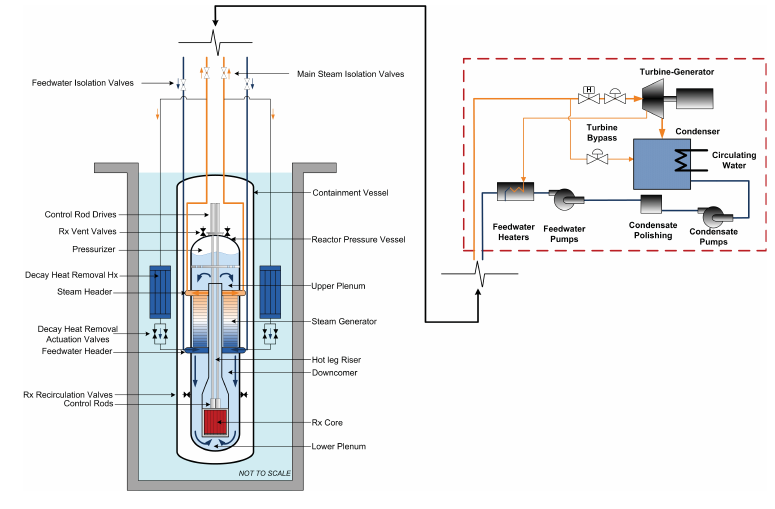
\includegraphics[scale=0.7]{Figs/nuscale2d.jpeg}
\caption{ Two-dimensional schematic of a single NuScale unit}
\label{Nu2d}
\end{figure}

\begin{figure}[htbp]
\centering
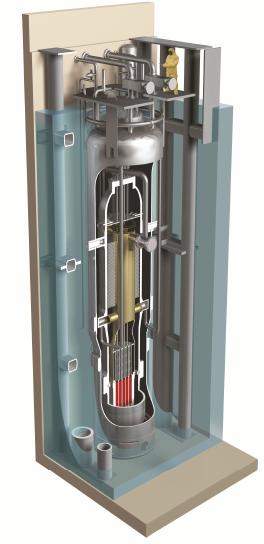
\includegraphics[scale=0.8]{Figs/nuscale3d.jpeg}
\caption{NuScale 3D SMR view}
\label{Nu3d}
\end{figure}

\pagebreak
\subsection{Oklo}
Oklo is working on a Compact Fast Reactor design since 2013. Oklo  is a 2  MWe  heat  pipe  reactor  (HPR),  cooled  by  sodium  heat  pipes,  fast  spectrum,  metallic  fuel (enrichment undisclosed). The reactor is designed to operate purely on natural physical forces, with very few moving parts. The core lifetime is up to 20 years before refueling. Very little information about this reactor is available directly from the company.

Since November 2016, NRC has been engaged in pre-application activities (the docket number - 99902046) with Oklo. Public version of the final safety analysis report of Oklo \cite{oklo_inc._pilot_2018} is not enough for the understanding of the reactor design. Full version has details such as probabilistic risk assessment, release pathway and environmental impact but was closed to public access. Even company web site is unreachable. The company is now making collaboration with ANL and INL. 

\subsection{Starcore}
The StarCore technical data is acquired directly from the vendor website and summarized in Table \ref{startable} below. In terms of size and basic technical characteristics, the reactor, illustrated in Fig \ref{Starcore}, is similar to HTR-10, a prototype pebble bed modular reactor built and operated in China, and HTTR, a 30 MWth experimental gas cooled reactor in Japan.

HTGR reactor with 2 reactor units per standard plant is embedded 15m underground in \gls{UHSC} silos. The reactors are installed in silos 57 meters deep (as seen in Fig. \ref{Starview}) and 13 meters in diameter, made from double-walled high performance concrete with a steel canister silo at the base.  TRISO fuel compacts supplied by BWX Technologies. StarCore is fully automated and has only two operating states: Load Following and Shutdown.

\begin{figure}[htbp]
\centering
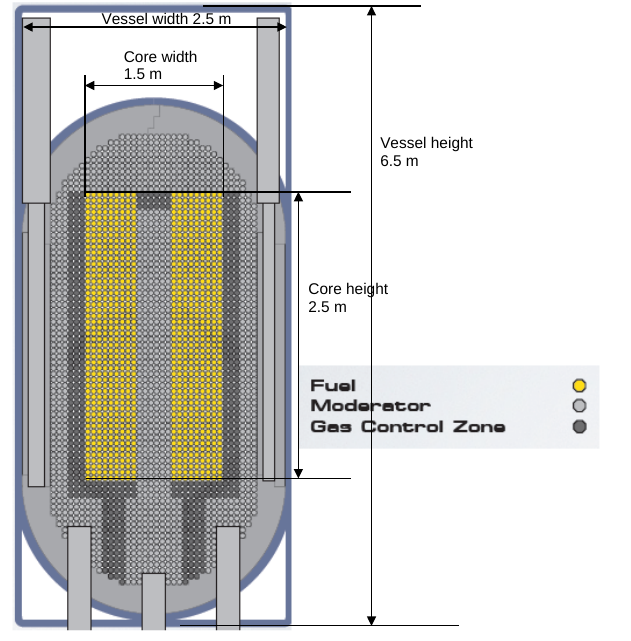
\includegraphics[scale=0.5]{Figs/starcorereactor.jpeg}
\caption{StarCore reactor core}
\label{Starcore}
\end{figure}

\begin{figure}[htbp]
\centering
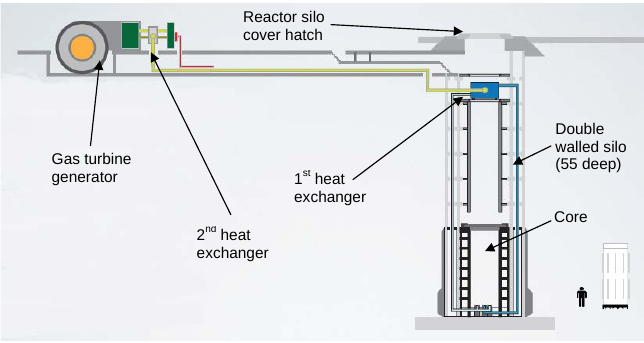
\includegraphics[scale=0.7]{Figs/starcoreview.jpeg}
\caption{Side view of Starcore}
\label{Starview}
\end{figure}

\begin{table} [ht]
\begin{center}

\caption{StarCore reactor design}
\label{startable}
\begin{tabular}{l l}
\hline 
Design 		&Value \\ 
\hline 
Core Diameter (m) 		&1.5 \\ 
Core Height (m) 		&2.5 \\ 
Refueling (y)		&  5 (off-site)\\ 
Fuel		&UCO TRISO Pebbles \\ 
Enrichment (\%)		&$<$20 \\ 
Number of fuel pebbles		&26,800 \\ 
Number of TRISO particles per pebble		&2,000 \\ 
Pebble fuel core diameter (mm)		&60 \\ 
Fuel element geometry & Truncated cuboctahedron\\ 
Cladding material & Silicon carbide \\ 
Primary side coolant 	&Helium \\ 
Core outlet temp ($^\circ{}$C) 	&850 \\ 
Core operating pressure (MPa)	&7.5 \\ 
Secondary side coolant	&Nitrogen \\ 
Secondary side operating pressure (MPa)	&6.8 \\ 
\hline 

\end{tabular}
\end{center}
\end{table}

\pagebreak
\subsection{Urenco}
The concept design, namely U-battery, has been made by the Universities of Manchester, Dalton Institute (UK) and Technology University of Delft (Netherlands). There is strong desire to operate the reactor by 2026. Main design parameters \cite{ding_design_2011} are tabulated in Table \ref{Utable}. A 3D view and core layout of the reactor are displayed in Figs. \ref{u3d} and \ref{ucore}. 

The coolant is pressurized He, the secondary side is cooled by nitrogen. It provides up to 750 $^\circ{}$C process heat. The power conversion is not specified.

\begin{table} [htbp]
\begin{center}

\caption{U-battery design}
\label{Utable}
\begin{tabular}{l l l}
\hline 
Design 		&10 MWe &20 MWe\\ 
\hline 
Reflector composition & BeO          &  Graphite\\
Control rods (\#) & 4                        &  6 \\
Fuel Blocks (\#) & 6*4                     & 30*4 \\
Enrichment (\%) & 20                      & 17  \\
Fuel life time (a)&  5                       & 10  \\
Fuel block dimension (cm) & 36*80 &  36*80 \\
Fuel mass (kg) & 208                     &   1.040\\
Burn-up (MWd/kg HM)  & 88           &   70 \\
\hline 
Outer diameter (cm)             &   180  &  370   \\
Vessel thickness (mm)        &   $<$100       & 100   \\
Reactor core diameter (cm)  &   108     &  252  \\
Reflector thickness (cm)      &   20 (BeO)    &29    \\
Insulation thickness (cm)     &   5 (SiC fiber)     & 10 (SiC fiber)   \\
Barrel thickness (cm)           &    2   & 2    \\
Gap thickness (cm)             &    5  &  5  \\
\hline 
Core Height (cm)          & 320         & 320 \\
Top reflector (cm)         &  20 (BeO)&50  \\
Bottom reflector (cm)    &  20 (BeO)& 50 \\
Top plenum (cm)          &20            &20  \\
Bottom plenum (cm)     &  50          &50  \\
Top insulation (cm)       &30           &30 \\
Bottom insulation (cm)  &  60         &60 \\
Core support plate (cm) &  10         &15  \\
Support structure (cm)  &   60         &60  \\
Vessel height (cm)       & 590         &655  \\
\hline 
BeO mass (kg) &    7.900       &0  \\
Graphite mass (kg) &   8.100        & 70.000  \\
Flask inner diam (cm)& 180       & - \\
Flask inner height (cm)& $<$500         & - \\
\hline 

\end{tabular}
\end{center}
\end{table}


\begin{figure}[htbp]
\centering
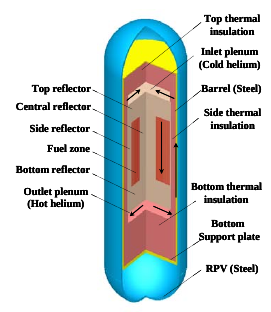
\includegraphics[scale=1]{Figs/ubattery3d.jpeg}
\caption{ 3D reactor configuration of U-battery}
\label{u3d}
\end{figure}

\begin{figure}[htbp]
\centering
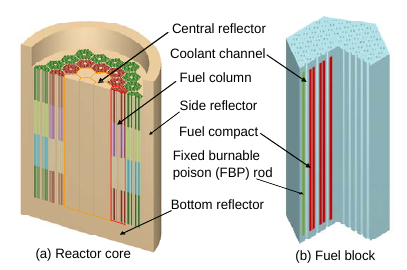
\includegraphics[scale=1]{Figs/ubatterycore.jpeg}
\caption{ Core and fuel block of U-battery}
\label{ucore}
\end{figure}


\pagebreak
\subsection{Terrestrial Energy}
Integral Molten Salt Reactor (IMSR) is 400 MWt / 195 MWe molten salt reactor (MSR), graphite-moderated, uranium salt fuel (~5\% enriched). The primary coolant is forced circulation fluoride salt with dissolved fuel, system pressure ~0.4 MPa (hydrostatic), core inlet/outlet temperatures 660/700 $^\circ{}$C. The IMSR is a sealed reactor vessel with integrated pumps, heat exchangers and shutdown rods all mounted inside a single vessel. The sealed core-unit is replaced at the end of its useful service life (nominally 7 years). The power conversion is a conventional steam cycle.

\subsection{USNC}
MMR(Micro Modular Reactor)a 15 MWt/ 5 MWe gas cooled reactor (GCR),  graphite  moderated,  TRISO  fuel  (enrichment 9-12\%)  in  a  prismatic  graphite  block. The  coolant  is natural convection helium, the intermediate heat transfer loop is molten salt, outlet temperature 640 $^\circ{}$C. The core lifetime is 20 years, with no refueling. The power conversion is not specified.

\pagebreak
\subsection{X-energy}
X-energy company provides various reactor designs ranging from 600 MWt to 30 MWt, called Pebble Bed Fuel Reactor. The main microreactor design is ST-OTTO (referring to Fig.  \ref{xo}) which produces 30-48 MWt power. But the design details are not open to the public. I think the design is very identical to the design of 200 MWt, as presented in Table \ref{xtable} except for the reactor size and fuel type. Th-based fuel is under consideration for the use in TRISOs. 

\begin{table} [ht]
\begin{center}

\caption{ X-energy design}
\label{xtable}
\begin{tabular}{l l}
\hline 
Design 		&Value \\ 
\hline 
RPV diameter (m) 		&4.88 \\ 
RPV height (m) 		&20 \\ 
Refueling		&Online fuel loading  \\ 
	&175 fresh pebbles/day \\ 
Fuel		&UCO TRISO Pebbles \\ 
Enrichment (\%)		&15.5 \\ 
Number of fuel pebbles		&220,000 \\ 
Number of TRISO particles per pebble		&18,000 \\ 
Pebble fuel core diameter (mm)		&50 \\ 
Pebble diameter (mm)	&60 \\ 
Number of passes		&6\\ 
Final burnup (GWd/tHM)		&160 \\ 
Burnable poison		&no \\ 
Power density (MW/m$^3$)		&4.8 \\ 
UCO TRISO kernel diameter (mm)	&0.425 \\ 
Porous Carbon Buffer thickness (mm)	&0.095 \\ 
Inner Pyrolytic Carbon Layer thickness (mm) 	&0.04 \\ 
Silicon Carbide Layer thickness (mm)	&0.035 \\ 
Outer Pyrolytic Carbon Layer thickness (mm)	&0.04 \\ 
Core Inlet temp ($^\circ{}$C)	&259 \\ 
Core Outlet temp ($^\circ{}$C) 	&750 \\ 
Core Inlet Pressure (MPa)	&6 \\ 
Core Outlet Pressure (MPa)	&5.84 \\ 
\hline 

\end{tabular}
\end{center}
\end{table}

\begin{figure}[hbtp]
\centering
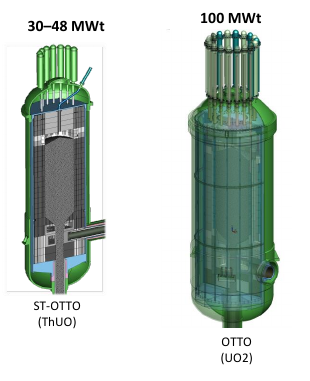
\includegraphics[scale=0.97]{Figs/xoverview.jpeg}
\caption{X-energy micro-reactor overview}
\label{xo}
\end{figure} 

\subsection{Westinghouse}
Full design details have not been revealed yet to the public; only general information is given by the company. However, general characteristic of eVinci is a 5 MWt / 2 MWe heat pipe reactor (HPR), cooled by sodium heat pipes, TRISO fuel (19.75 \% enriched) in  a  solid graphite block  core. It  can  produce  up  to  600 $^\circ{}$C  process  heat, the  waste  heat  is  rejected  to  the atmosphere.  The  core lifetime is 10 years.  It  is  factory  built,  assembled,  fueled,  and  tested, and transported to  the deployment site. The power conversion is not specified.

Several academic studies, most of them eVinci-like, can be found in the literature. Recently, two papers, \cite{hong_thermal_2019} and \cite{wright_phenomena_2019}, have been published in 18th \gls{NURETH} conference. Those are not available for now but reaching them somehow would be valuable. Westinghouse is planning to finalize the current design of eVinci by 2022, testing by 2023 and commercializing by 2025. Hernandez et al. \cite{hernandez_micro_2019} performed a series of calculations in eVinci-like (not eVinci) for natural resource utilization, burnup analyses, waste management and environmental impacts. The details of eVinci design obtained from the documents published by Westinghouse are presented in Table 3. Reactor core configuration and 3D design representation are given in Figs. \ref{eVincidesign} and \ref{eVincioverview}.

\begin{table} [ht]
\begin{center}

\caption{eVinci design parameters}
\begin{tabular}{l  l  l}
\hline
Design 		&Value (from Westinghouse reports) 		& Value (other) \cite{hernandez_micro_2019}\\ 
	& 	\cite{iaea_advances_2018};\cite{levinsky_westinghouse_2018};\cite{yan_technology_2020};\cite{arafat_evinci_2019} 	&  \\ 
\hline
Core Diameter (in) 		&59.06 		&  \\ 
Monolith materials 		& 		& Type-316 SS	\\ 
Refueling (years) 		&Up to 10 		&  \\ 
Fuel 		&UN/U-Mo 		& 	 \\ 
Fuel Pellet Density, \% TD 		&96 		&  \\ 
Enrichment (\%) 		&19.75 		&  \\ 
Fuel channel radius (in) 		& 		& 0.281 \\ 
Number of fuel channels 		&378 (1 MWth), 4219 (14 MWth)		& 2112 (5 MWth) \\ 
Reflector material 		&		& BeO\\ 
\gls{HP} channel radius (in) 		&		& 0.298\\ 
Number of HP channels 		& 		& 1224\\ 
HP to HP web thickness (in) 		& 		& 0.039\\ 
Fuel to fuel web thickness (in) 		& 		& 0.059\\ 
HP total length (ft) 		&		& 13.12\\ 
HP fluid 		&Na/K		& \\ 
HP fluid temperature (K) 		&920 		& \\ 
\hline

\end{tabular}
\end{center}
\end{table}

\begin{figure}[hbtp]
\centering
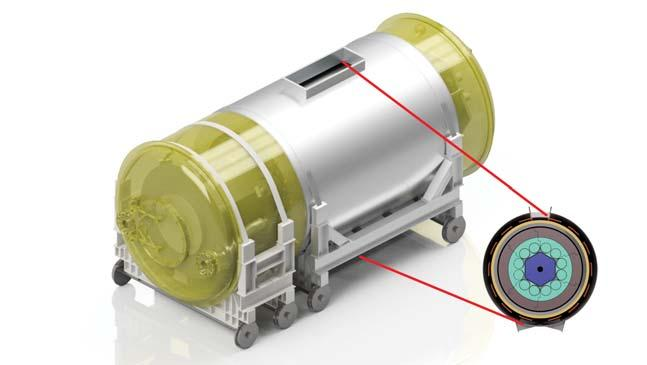
\includegraphics[scale=0.5]{Figs/evincicore.jpeg}
\caption{eVinci Core Configuration}
\label{eVincidesign}
\end{figure}

\begin{figure}[hbtp]
\centering
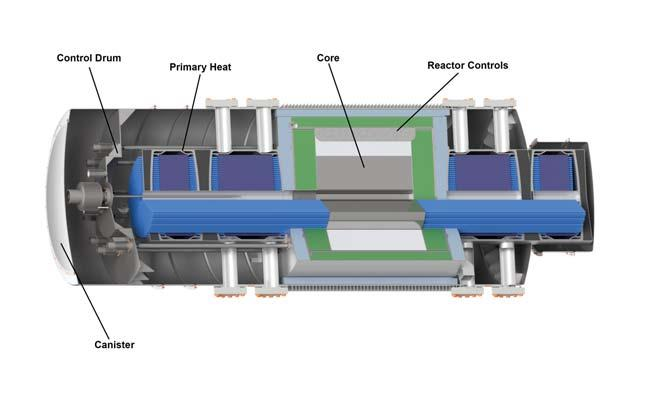
\includegraphics[scale=0.5]{Figs/evinciover.jpeg}
\caption{eVinci Micro Reactor Overview}
\label{eVincioverview}
\end{figure}

\pagebreak
